% !TeX root = main.tex
\chapter{Experimental Setup}
\label{ch:data}

This chapter describes the data and the setup of the experiments to fulfill the \glspl{rq}. Section~\ref{sec:datasets} introduces the eleven datasets and their roles, and Section~\ref{metrics} defines the evaluation metrics. Section~\ref{sec:training-setup} then gives the training settings of the pipelines, Section~\ref{sec:page-selection-setup} the page selection of the page-count study, and Section~\ref{sec:cross-generalization} the setup of the cross-generalizatio  experiments.

\section{Datasets}
\label{sec:datasets}\label{sec:data-benchmarks}\label{sec:data-pretraining}\label{sec:data-cross}

The experiments use eleven historical document datasets. DIVA-HisDB and U-DIADS-TL with published results are used to compare the pipelines, encoders, and initializations and to study the number of training pages. Two larger collections are used for the initializations: CATMuS Medieval for supervised pretraining and cBAD 2019 for unsupervised knowledge distillation~\cite{beyer2022knowledgedistillationgoodteacher} with DINOv3 as the teacher model. The remaining seven collections form the pool for the cross-generalization experiments. Table~\ref{tab:dataset-splits} gives the number of training, validation, and test pages of each dataset. For U-DIADS-TL and DIVA-HisDB, the counts refer to each manuscript, and the partition of the seven cross-collection datasets is described in Section~\ref{sec:data-partitions}.

\begin{table}[htbp]
    \centering
    \caption{Datasets used in the experiments.}
    \label{tab:dataset-splits}
    \scriptsize
    \setlength{\tabcolsep}{3.5pt}
    \renewcommand{\arraystretch}{0.82}
    \captionsetup{font=footnotesize,skip=2pt}
    \begin{tabularx}{\textwidth}{@{}>{\raggedright\arraybackslash}p{3.0cm} >{\raggedright\arraybackslash}p{3.2cm} >{\centering\arraybackslash}p{2.4cm} >{\raggedright\arraybackslash}X@{}}
        \toprule
        Dataset & Language or script & Train/val/test & Text line ground truth \\
        \midrule
        U-DIADS-TL \cite{Zottin_2025_FEST} & Latin, Syriac & 3/10/15 & Binary pixel-level line masks \\
        DIVA-HisDB \cite{diva_hisdb} & Latin, Italian & 20/10/10 & PAGE XML line polygons \\
        CATMuS Medieval \cite{catmus-medieval} & Multilingual Latin script & 1335/191/-- & PAGE XML line polygons \\
        cBAD 2019 \cite{cbad-2019,DiemKleberGatos2019} & Multilingual European collections & 755/755/1511 & PAGE XML regions and baselines \\
        Pinkas \cite{Barakat2019Pinkas} & Hebrew & 3/3/6 & PAGE XML line polygons \\
        ONB Cod.\ Syr.\ 1 \cite{AboudIshac2025ONBSyr1} & Syriac & 3/14/123 & PAGE XML line polygons \\
        RASAM \cite{VidalGorene2021RASAM} & Arabic (Maghrebi) & 3/52/462 & PAGE XML line polygons \\
        RASM2018/2019 \cite{KeinanSchoonbaert2019RASM} & Arabic & 3/12/105 & PAGE XML line polygons \\
        Phil.\ gr.\ 130 \cite{SindlevAndersen2026PhilGrGT} & Medieval Greek & 3/2/13 & PAGE XML line polygons \\
        GRPOLY-DB \cite{Gatos2015GRPOLY} & Polytonic Greek & 3/5/38 & PAGE XML line polygons \\
        NorHand v3 \cite{Beyer2023NorHand} & Norwegian & 3/11/81 & PAGE XML line polygons \\
        \bottomrule
    \end{tabularx}
\end{table}

The two benchmarks use different \gls{gt} formats, binary line masks and line polygons (Figure~\ref{fig:gt-formats}), so every pipeline has to produce both:
\begin{itemize}
    \item \textbf{U-DIADS-TL}~\cite{Zottin_2025_FEST} is the benchmark of the ICDAR 2025 FEST competition. It contains 28 pages from each of the manuscripts Latin2, Latin14396, and Syriaque 341, annotated with binary pixel-level line masks. The validation pages are used only for model and postprocessing selection.
    \item \textbf{DIVA-HisDB}~\cite{diva_hisdb} contains 50 pages from each of Codex Bodmer 55 (CB55), Codex Sangallensis 18 (CS18), and Codex Sangallensis 863 (CS863), with main text, glosses, decorations, and overlapping lines. The experiments use the Task~2 PAGE XML annotations, which provide a polygon and a baseline for each text line.
\end{itemize}
The two initizalization corpora are much with 1,526 and 3,021 pages, but only CATMuS Medieval is annotated with line polygons (Figure~\ref{fig:initialization-datasets}):
\begin{itemize}
    \item \textbf{CATMuS Medieval}~\cite{catmus-medieval} contains medieval Latin-script manuscripts in Latin, French, Iberian, and Italian with PAGE XML line polygons, which are used for supervised pretraining.
    \item \textbf{cBAD 2019}~\cite{cbad-2019} contains pages from seven European archives, annotated with text regions and baselines but without line polygons. Only its page images are used, without labels, for representation distillation.
\end{itemize}
The seven cross-generalization datasets cover five scripts, Hebrew, Syriac, Arabic, Greek, and Latin, as well as different line densities and degrees of degradation (Figure~\ref{fig:rq3-collections}):
\begin{itemize}
    \item \textbf{Pinkas}~\cite{Barakat2019Pinkas} contains 30 pages of early-modern records of the Frankfurt Jewish community in Hebrew, with bleed-through, stains, faded ink, and overlapping lines. Three training pages without valid line polygons are excluded.
    \item \textbf{ONB Cod.\ Syr.\ 1}~\cite{AboudIshac2025ONBSyr1} contains 140 folios of a 16th-century Syriac manuscript of the Austrian National Library with one main-text column. Short, partly vertical marginal lines are annotated as separate lines.
    \item \textbf{RASAM}~\cite{VidalGorene2021RASAM} contains 517 pages from 18 Arabic manuscripts in Maghrebi scripts of the BULAC library, combining both released parts. The images are taken from the library's IIIF server, and the polygons are rescaled where the image resolution differs from the PAGE XML page size.
    \item \textbf{RASM2018/2019}~\cite{KeinanSchoonbaert2019RASM} contains 120 pages of Arabic scientific manuscripts from the 10th to the 19th century from the British Library, with 2,620 line polygons. Its pages measure up to \(6464\times8984\) pixels, the highest resolution in the pool.
    \item \textbf{Phil.\ gr.\ 130}~\cite{SindlevAndersen2026PhilGrGT} contains 18 pages of a 14th-century Greek manuscript of the Austrian National Library with 847 line polygons. The images are not part of the release and are taken from the library viewer. With about 47 lines per page, it is the densest collection in the pool.
    \item \textbf{GRPOLY-DB}~\cite{Gatos2015GRPOLY} is used only in its handwritten part: 46 pages of Greek polytonic documents with 693 line polygons. The pages contain few, widely spaced lines, and the polygons enclose a wide band around the handwriting.
    \item \textbf{NorHand v3}~\cite{Beyer2023NorHand} contains Norwegian letters and diaries from the 19th and early 20th centuries. The official test set is kept, and a random subset of 30 official training pages, drawn with seed 42, serves as the pool for training and validation pages. The line polygons range from narrow strips to irregular contours.
\end{itemize}

\begin{figure}[htbp]
    \centering
    \begin{subfigure}[t]{0.48\linewidth}
        \centering
        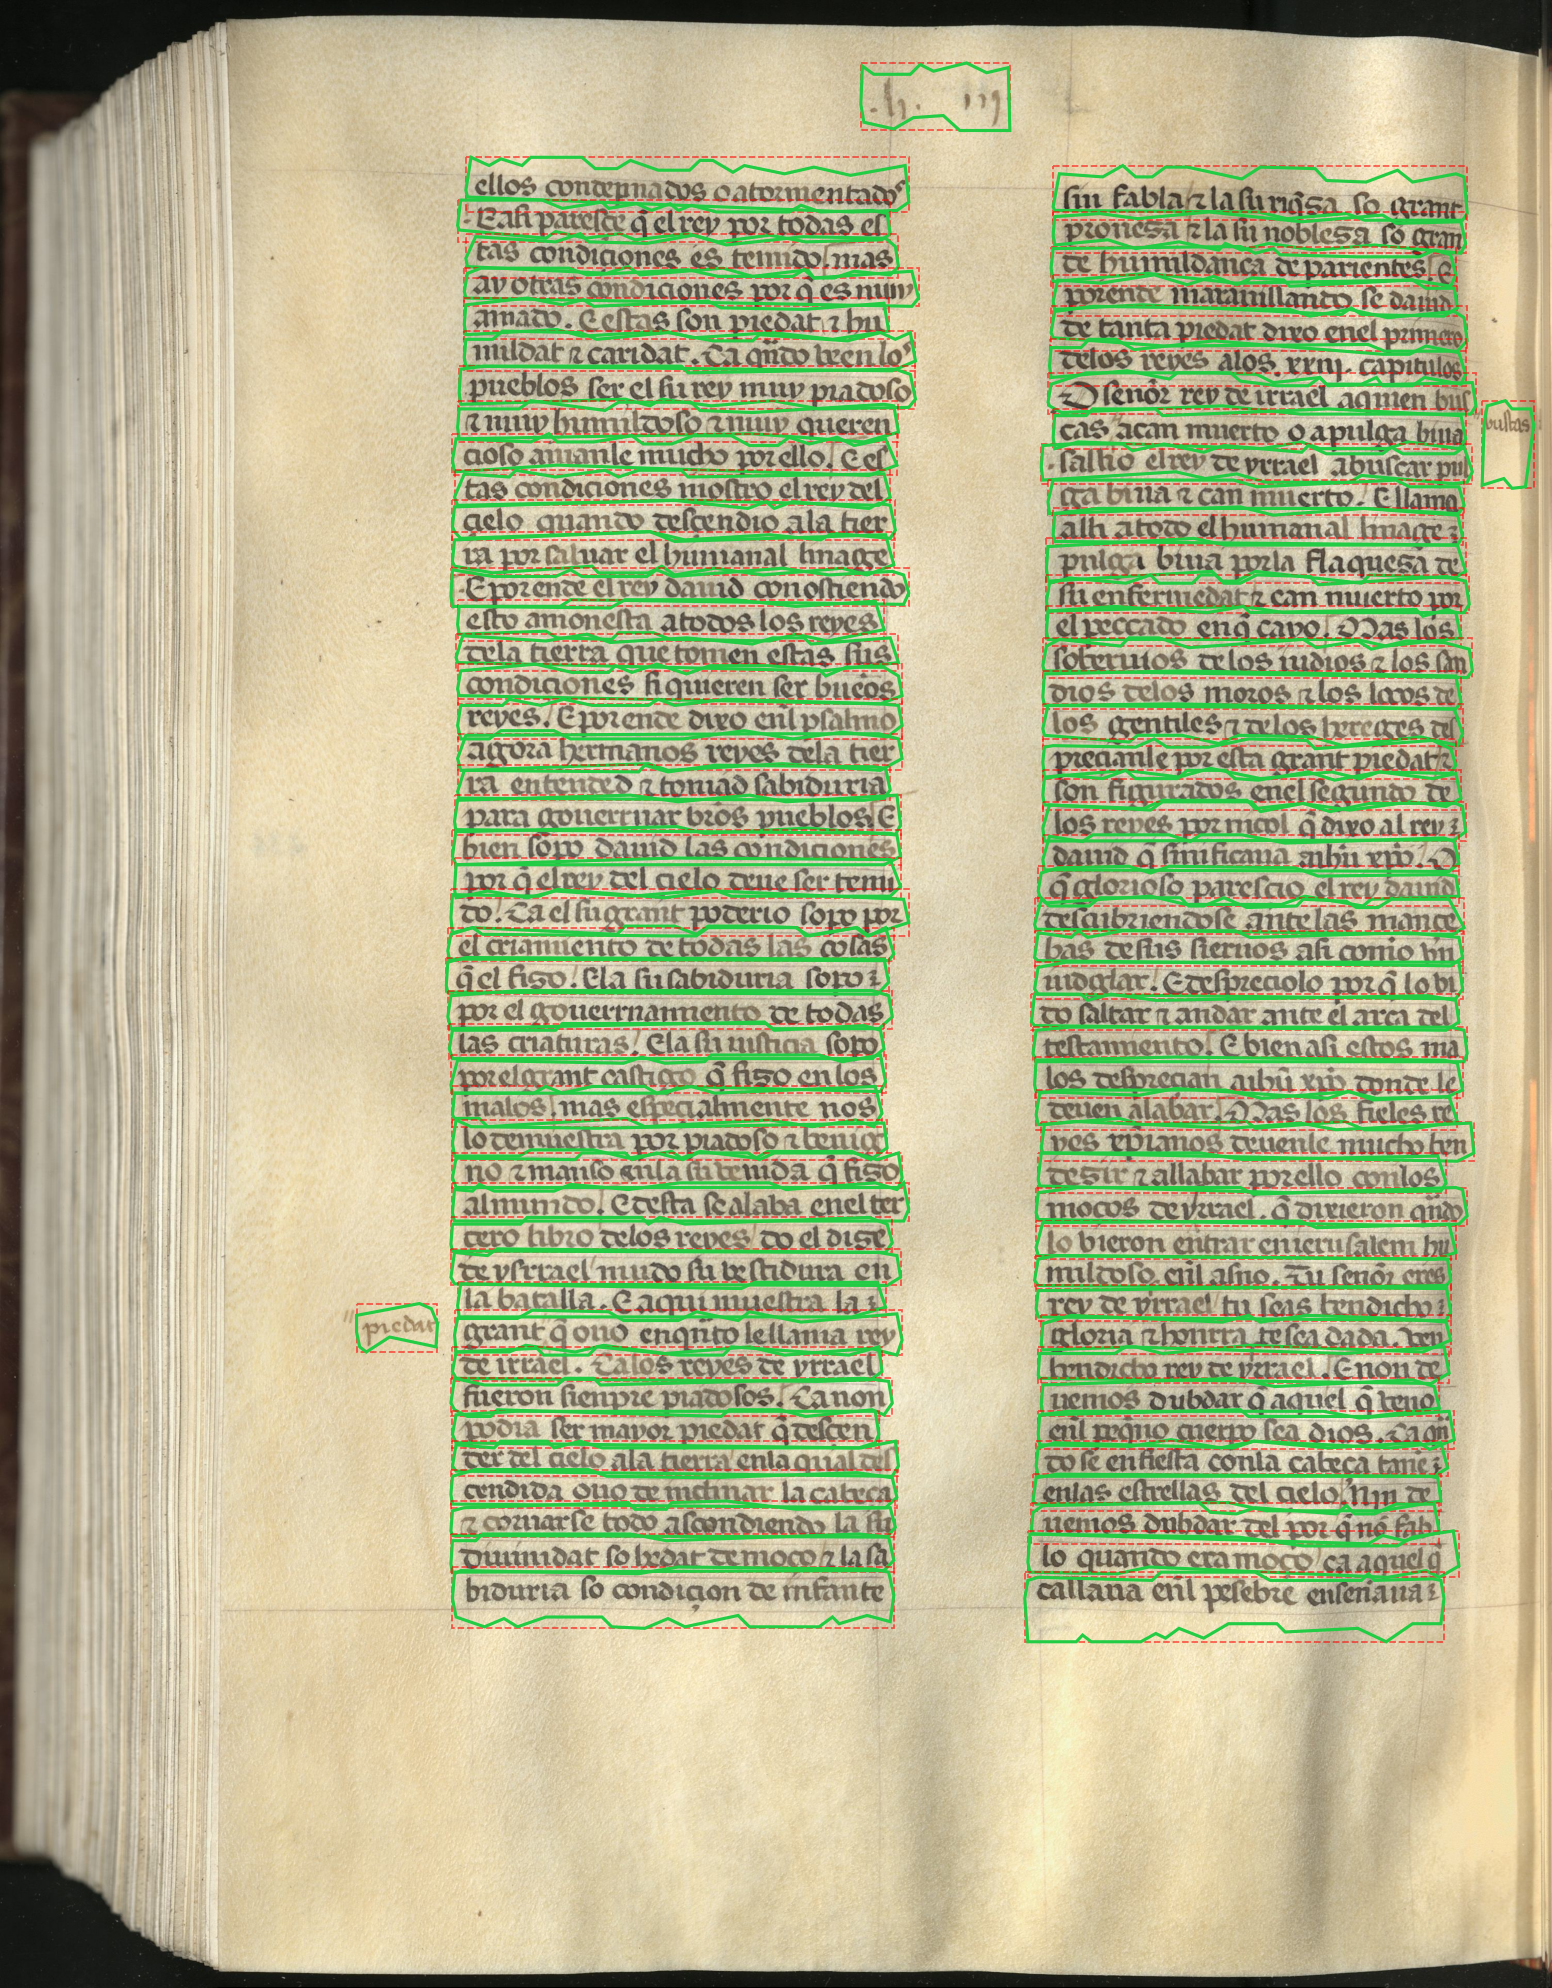
\includegraphics[width=\linewidth,height=0.42\textheight,keepaspectratio]{graphics/dataset_catmus_example.png}
        \caption{A CATMuS page with text-line polygons.}
    \end{subfigure}\hfill
    \begin{subfigure}[t]{0.48\linewidth}
        \centering
        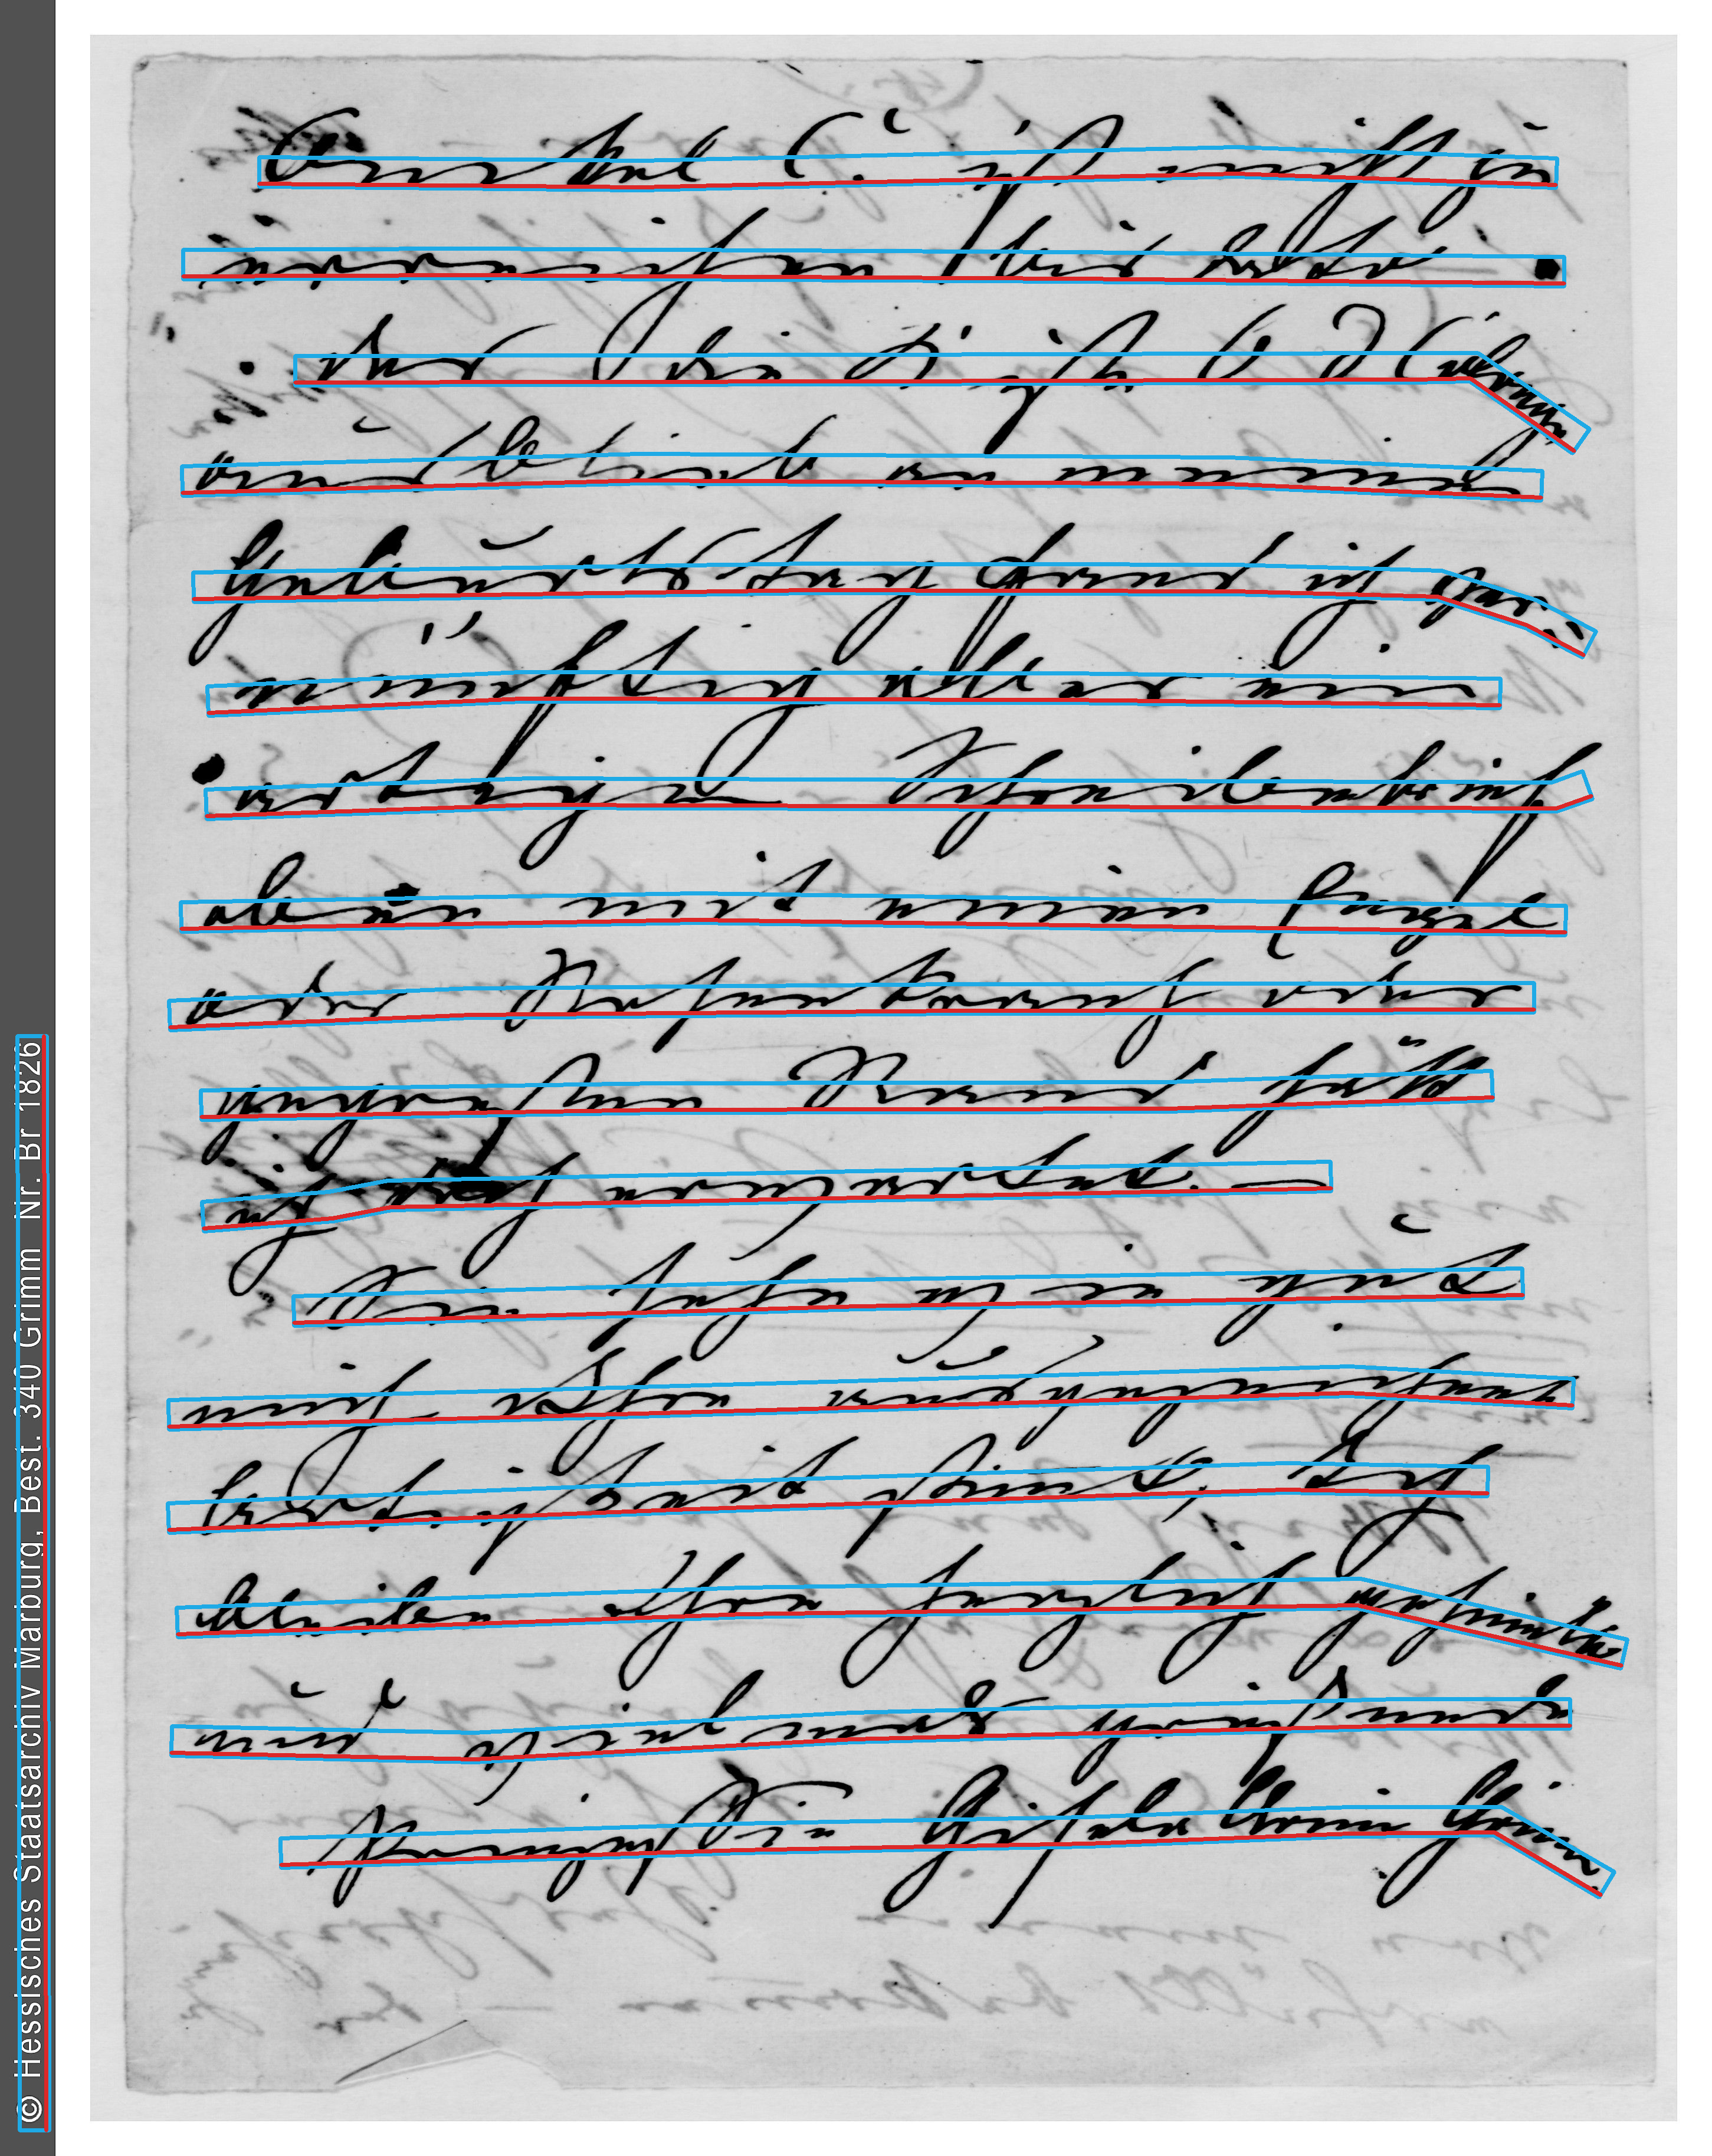
\includegraphics[width=\linewidth,height=0.42\textheight,keepaspectratio]{graphics/dataset_cbad_example.png}
        \caption{A cBAD page with region contours and baselines.}
    \end{subfigure}
    \caption{Example pages of the pretraining corpora CATMuS Medieval~\cite{catmus-medieval} and cBAD 2019~\cite{cbad-2019}.}
    \label{fig:initialization-datasets}
\end{figure}

\begin{figure}[htbp]
    \centering
    \begin{subfigure}[t]{0.49\linewidth}\centering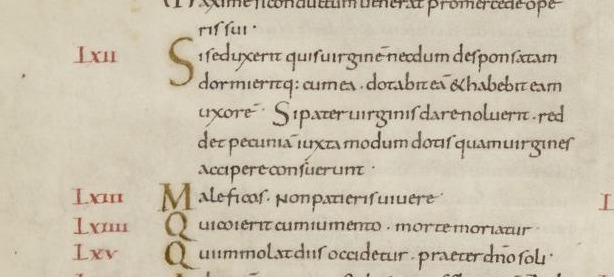
\includegraphics[width=\linewidth]{graphics/gtfmt_udiads_img.jpg}\caption{U-DIADS-TL page.}\label{fig:gt-formats-udiads}\end{subfigure}\hfill
    \begin{subfigure}[t]{0.49\linewidth}\centering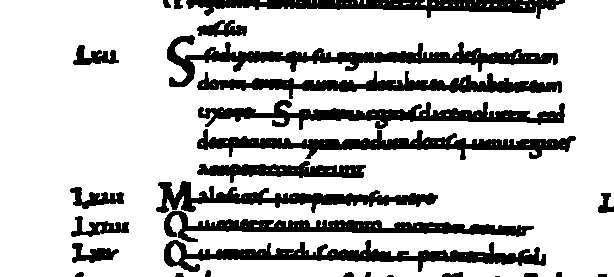
\includegraphics[width=\linewidth]{graphics/gtfmt_udiads_mask.png}\caption{U-DIADS-TL binary line mask.}\end{subfigure}\\[4pt]
    \begin{subfigure}[t]{0.49\linewidth}\centering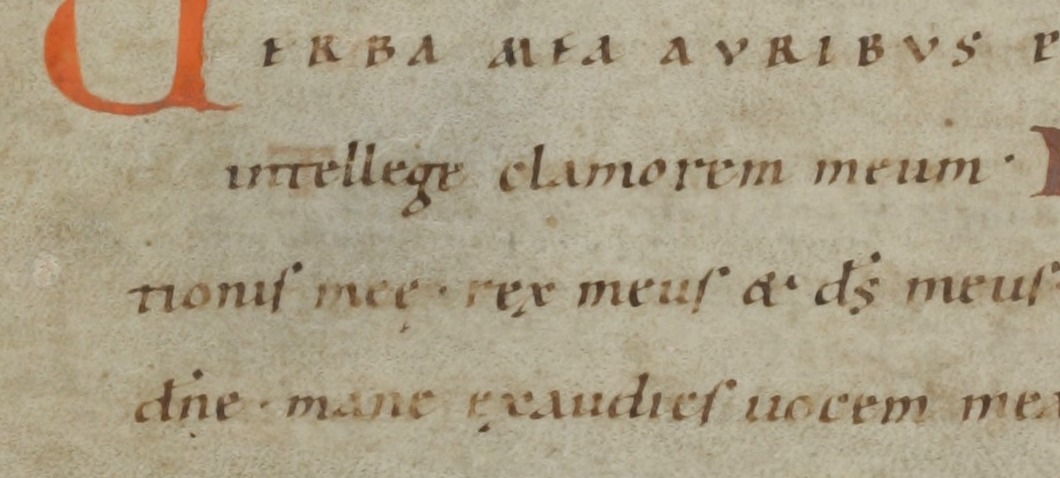
\includegraphics[width=\linewidth]{graphics/gtfmt_diva_img.jpg}\caption{DIVA-HisDB page.}\label{fig:gt-formats-diva}\end{subfigure}\hfill
    \begin{subfigure}[t]{0.49\linewidth}\centering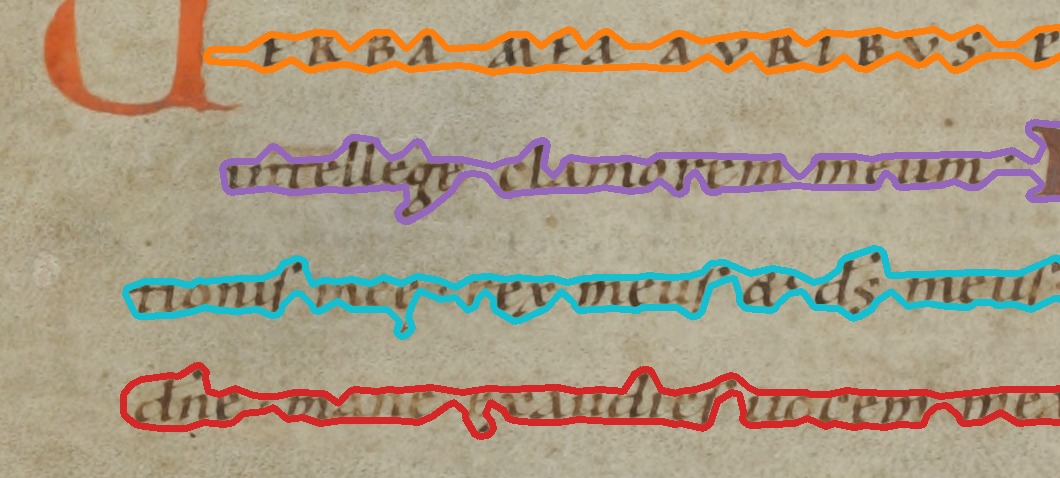
\includegraphics[width=\linewidth]{graphics/gtfmt_diva_polys.jpg}\caption{DIVA-HisDB line polygons.}\end{subfigure}
    \caption{Ground-truth formats: binary line mask with drawn baselines (U-DIADS-TL Latin2) and line polygons (DIVA-HisDB CS18). Generated from U-DIADS-TL~\cite{Zottin_2025_FEST} and DIVA-HisDB~\cite{diva_hisdb}.}
    \label{fig:gt-formats}
\end{figure}

\begin{figure}[htbp]
    \centering
    \begin{subfigure}[t]{0.32\linewidth}\centering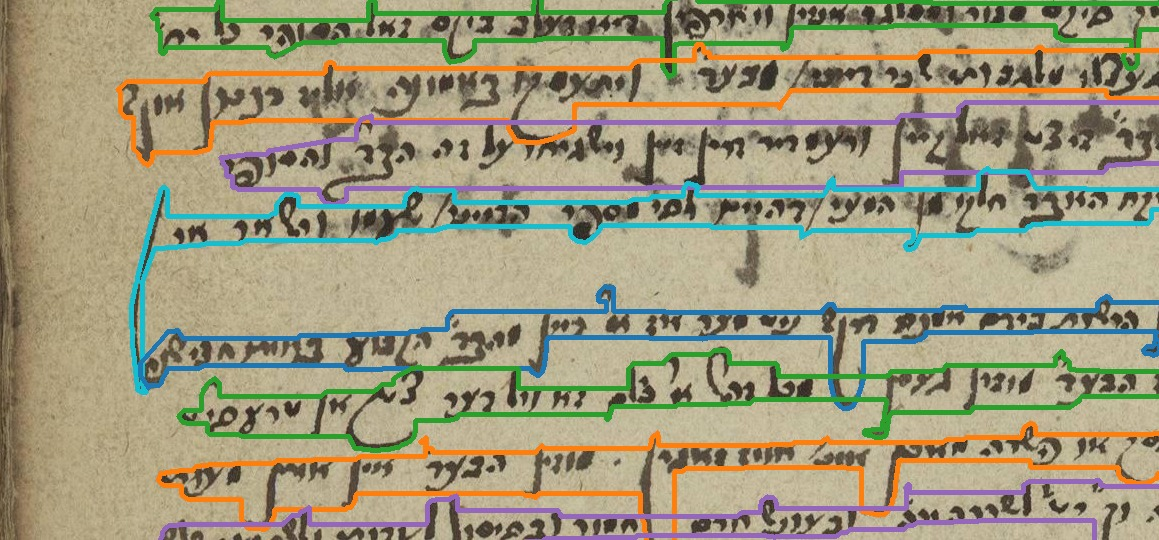
\includegraphics[width=\linewidth,height=4.2cm,keepaspectratio]{graphics/rq3gt_Pinkas.jpg}\caption{Pinkas.}\end{subfigure}\hfill
    \begin{subfigure}[t]{0.32\linewidth}\centering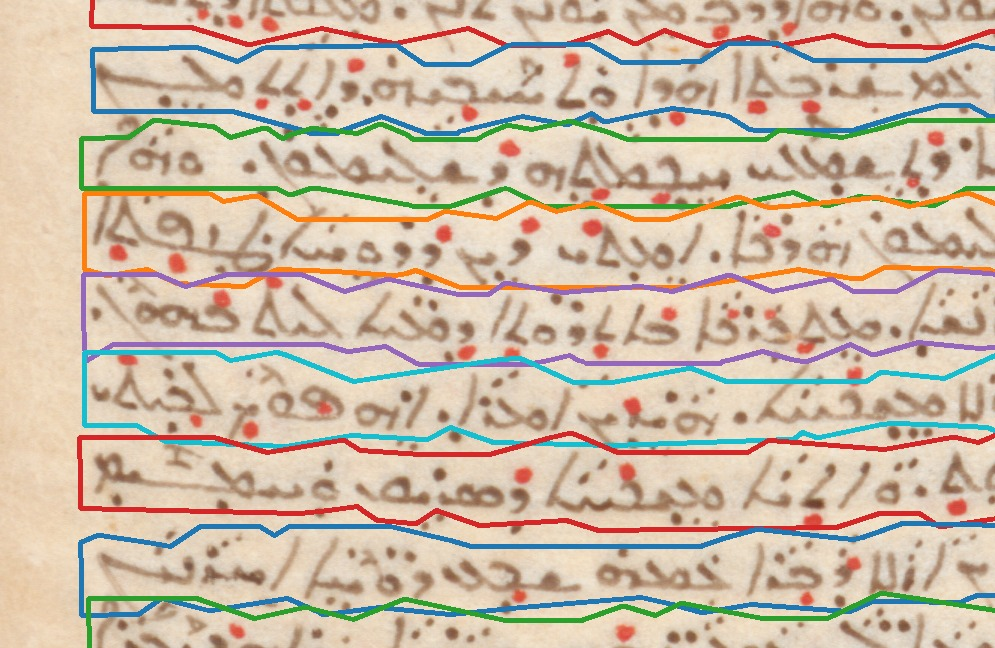
\includegraphics[width=\linewidth,height=4.2cm,keepaspectratio]{graphics/rq3gt_ONB.jpg}\caption{ONB Cod.\ Syr.\ 1.}\end{subfigure}\hfill
    \begin{subfigure}[t]{0.32\linewidth}\centering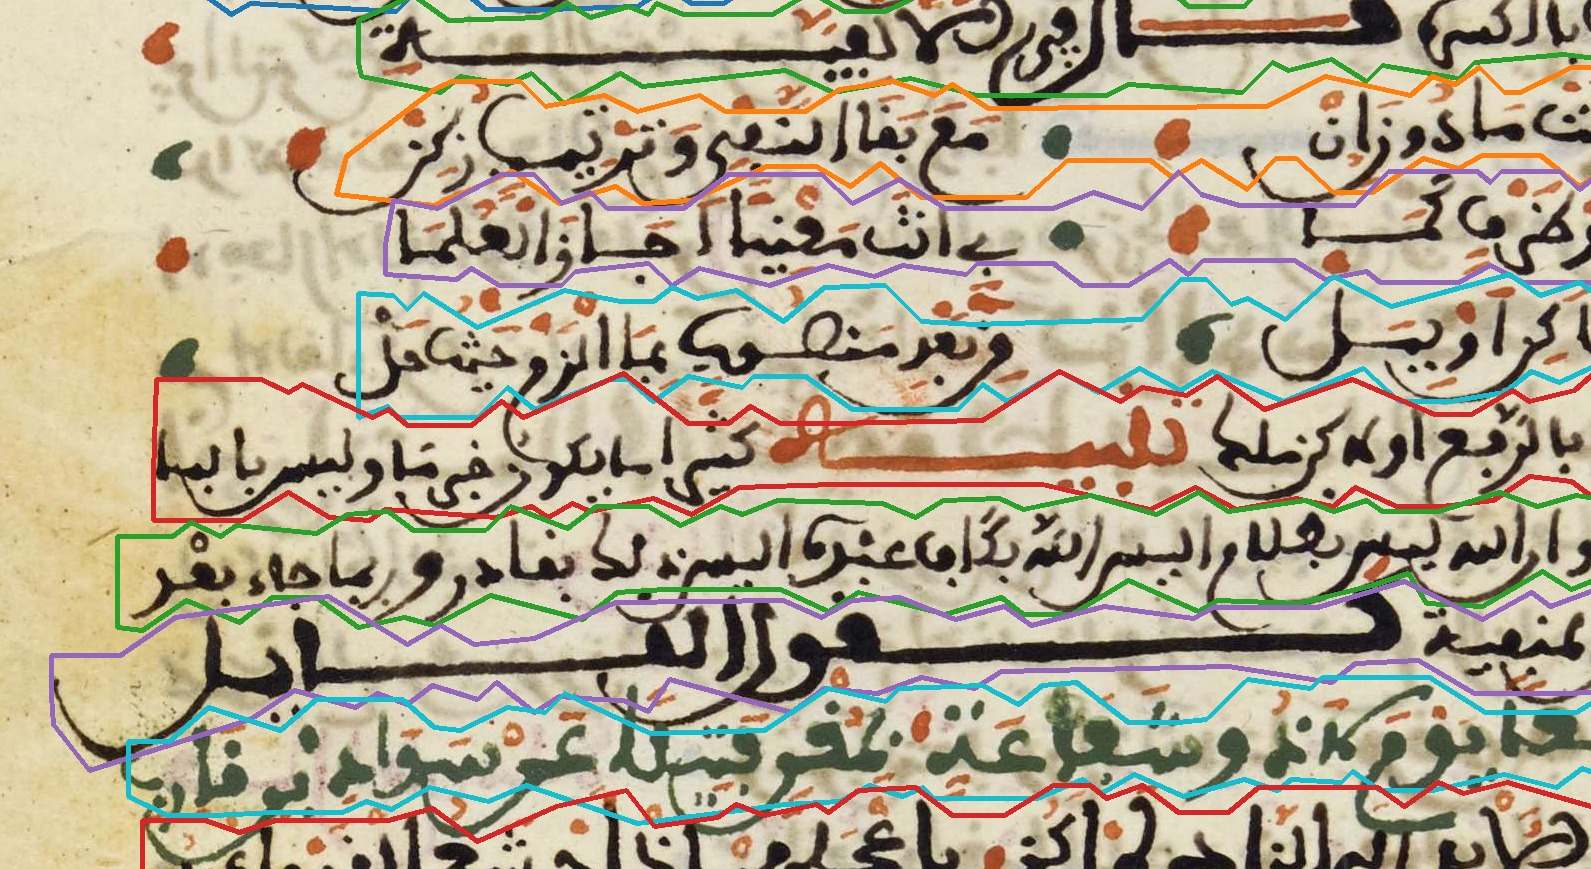
\includegraphics[width=\linewidth,height=4.2cm,keepaspectratio]{graphics/rq3gt_RASAM.jpg}\caption{RASAM.}\end{subfigure}

    \medskip
    \begin{subfigure}[t]{0.32\linewidth}\centering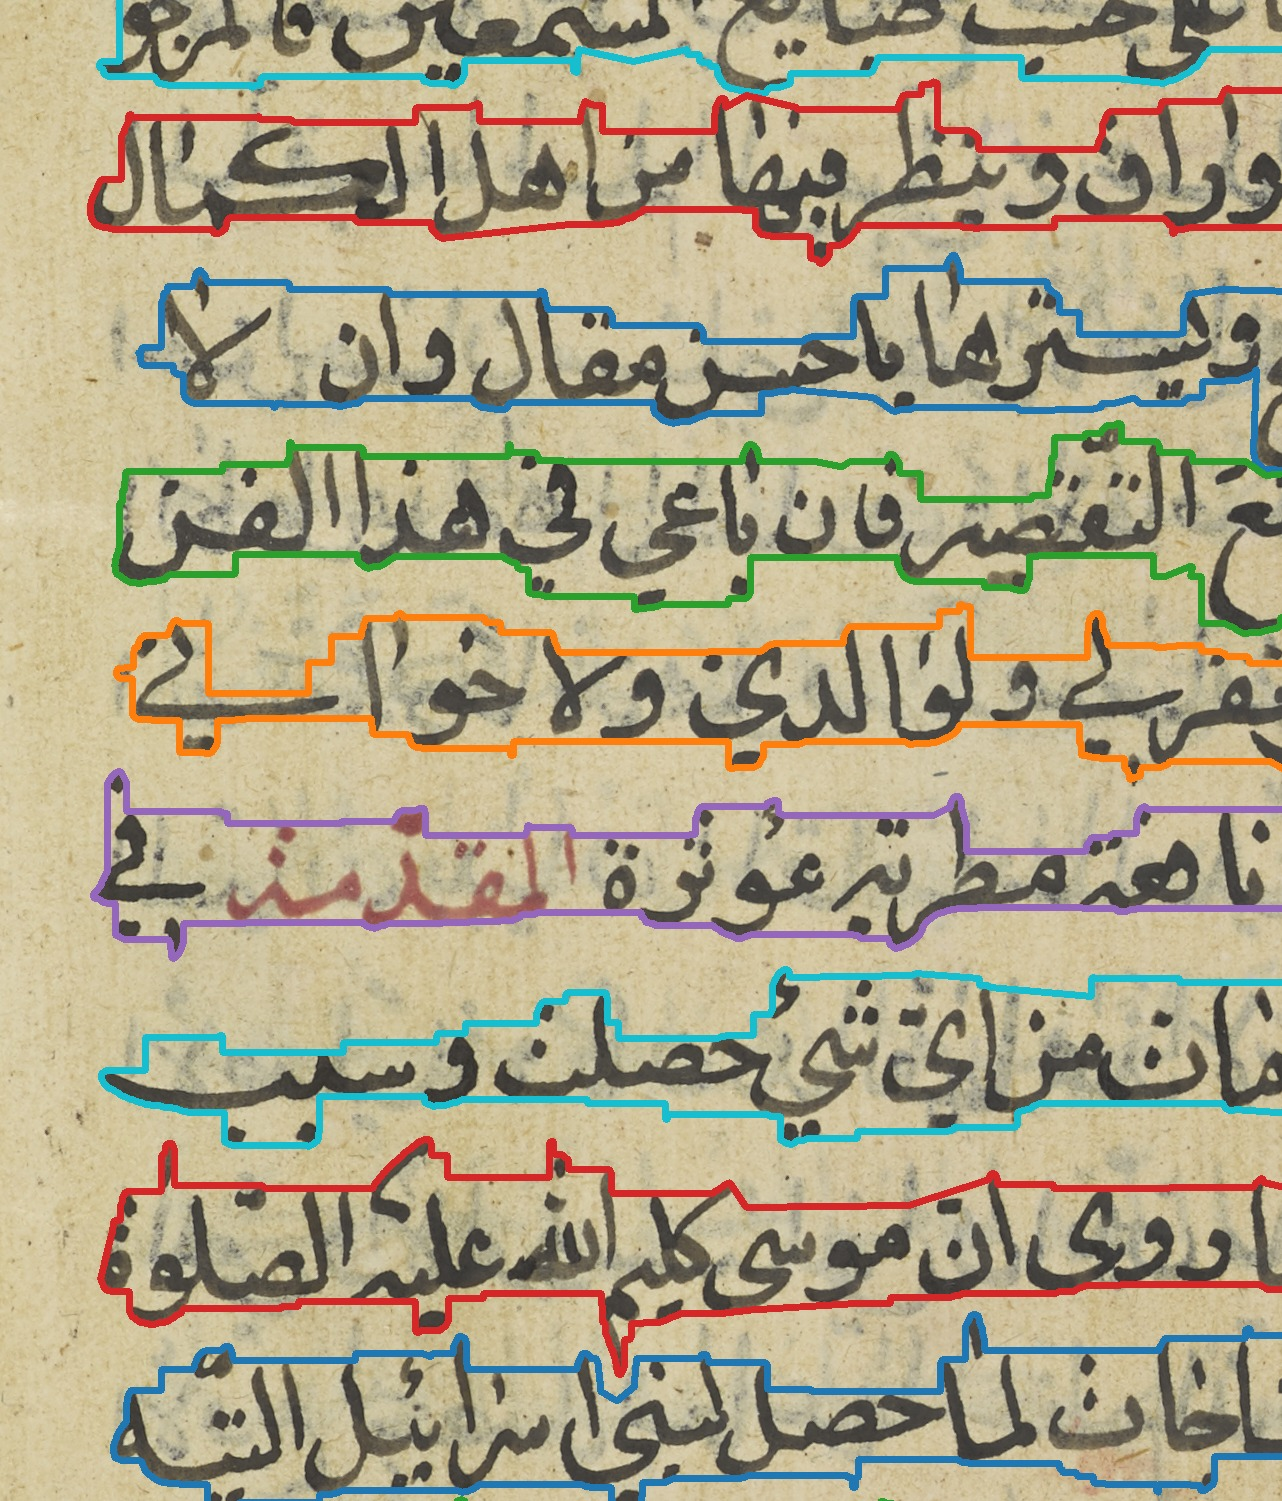
\includegraphics[width=\linewidth,height=4.2cm,keepaspectratio]{graphics/rq3gt_RASM.jpg}\caption{RASM2018/2019.}\end{subfigure}\hfill
    \begin{subfigure}[t]{0.32\linewidth}\centering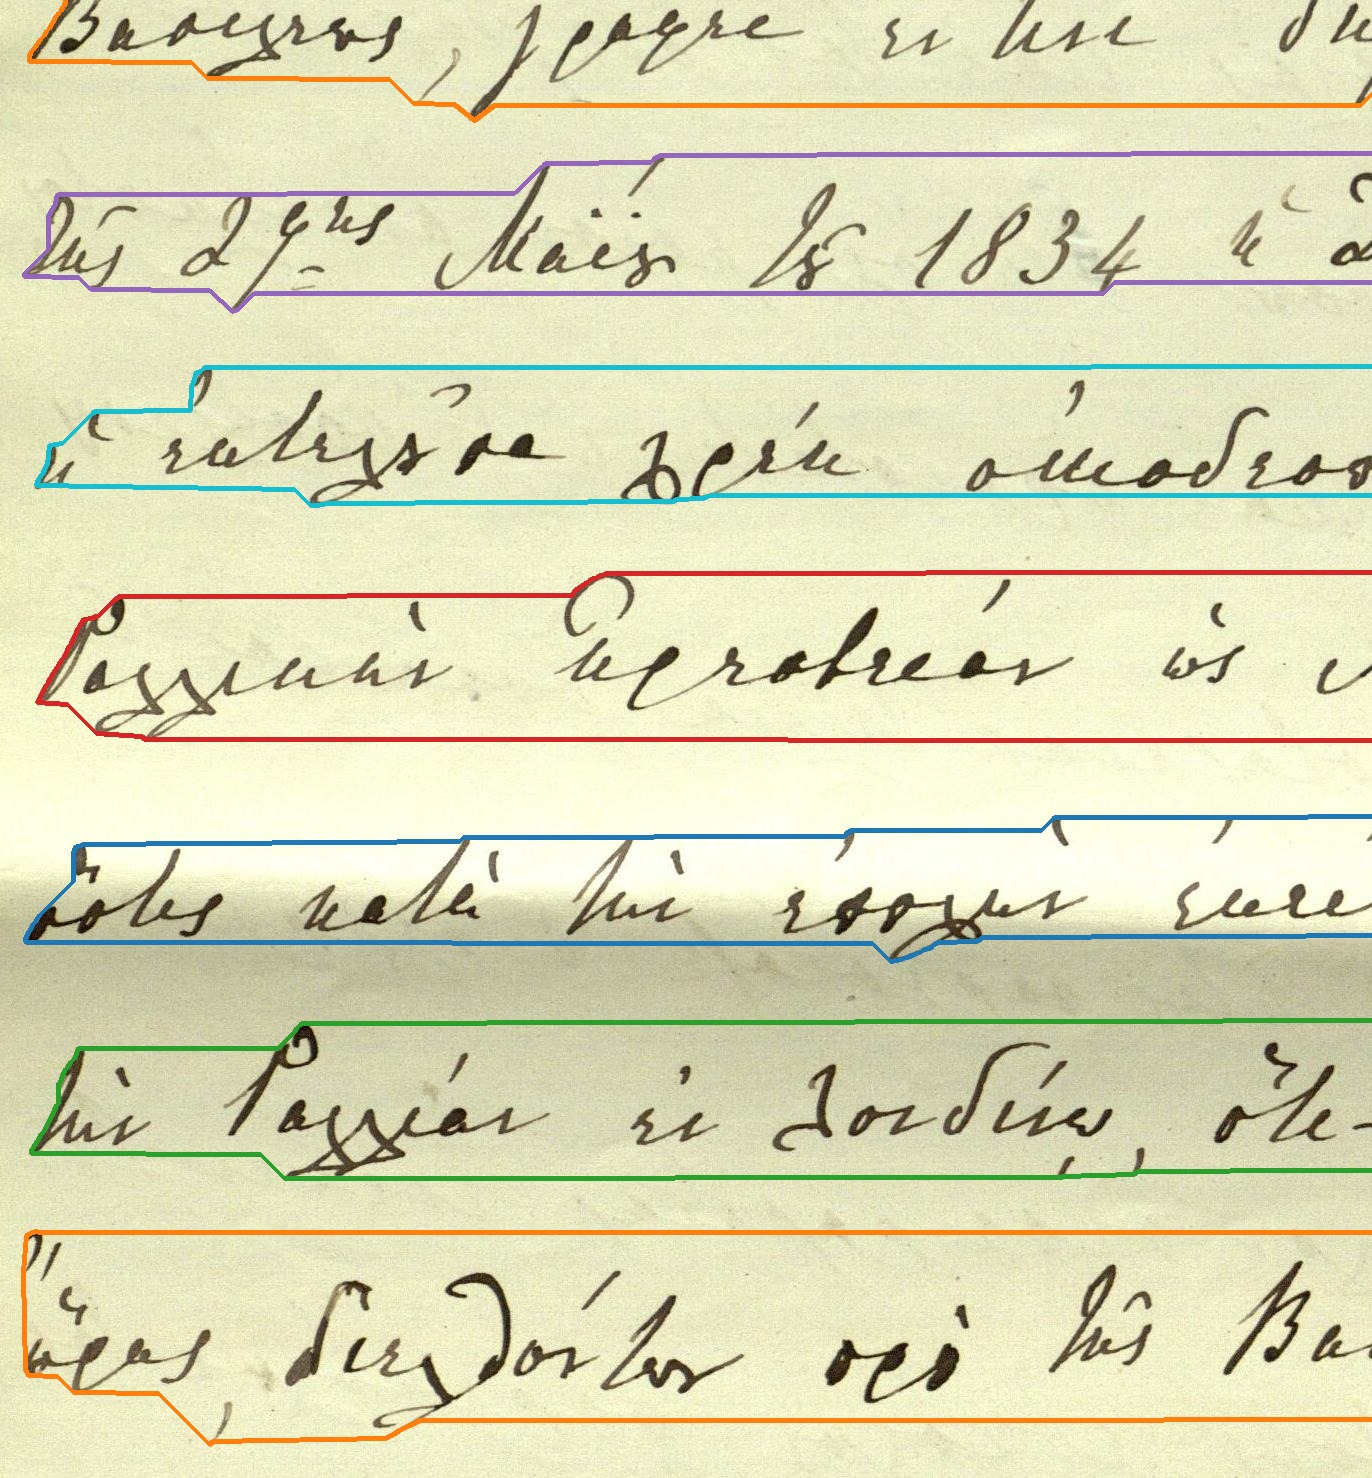
\includegraphics[width=\linewidth,height=4.2cm,keepaspectratio]{graphics/rq3gt_GRPOLY.jpg}\caption{GRPOLY-DB.}\end{subfigure}\hfill
    \begin{subfigure}[t]{0.32\linewidth}\centering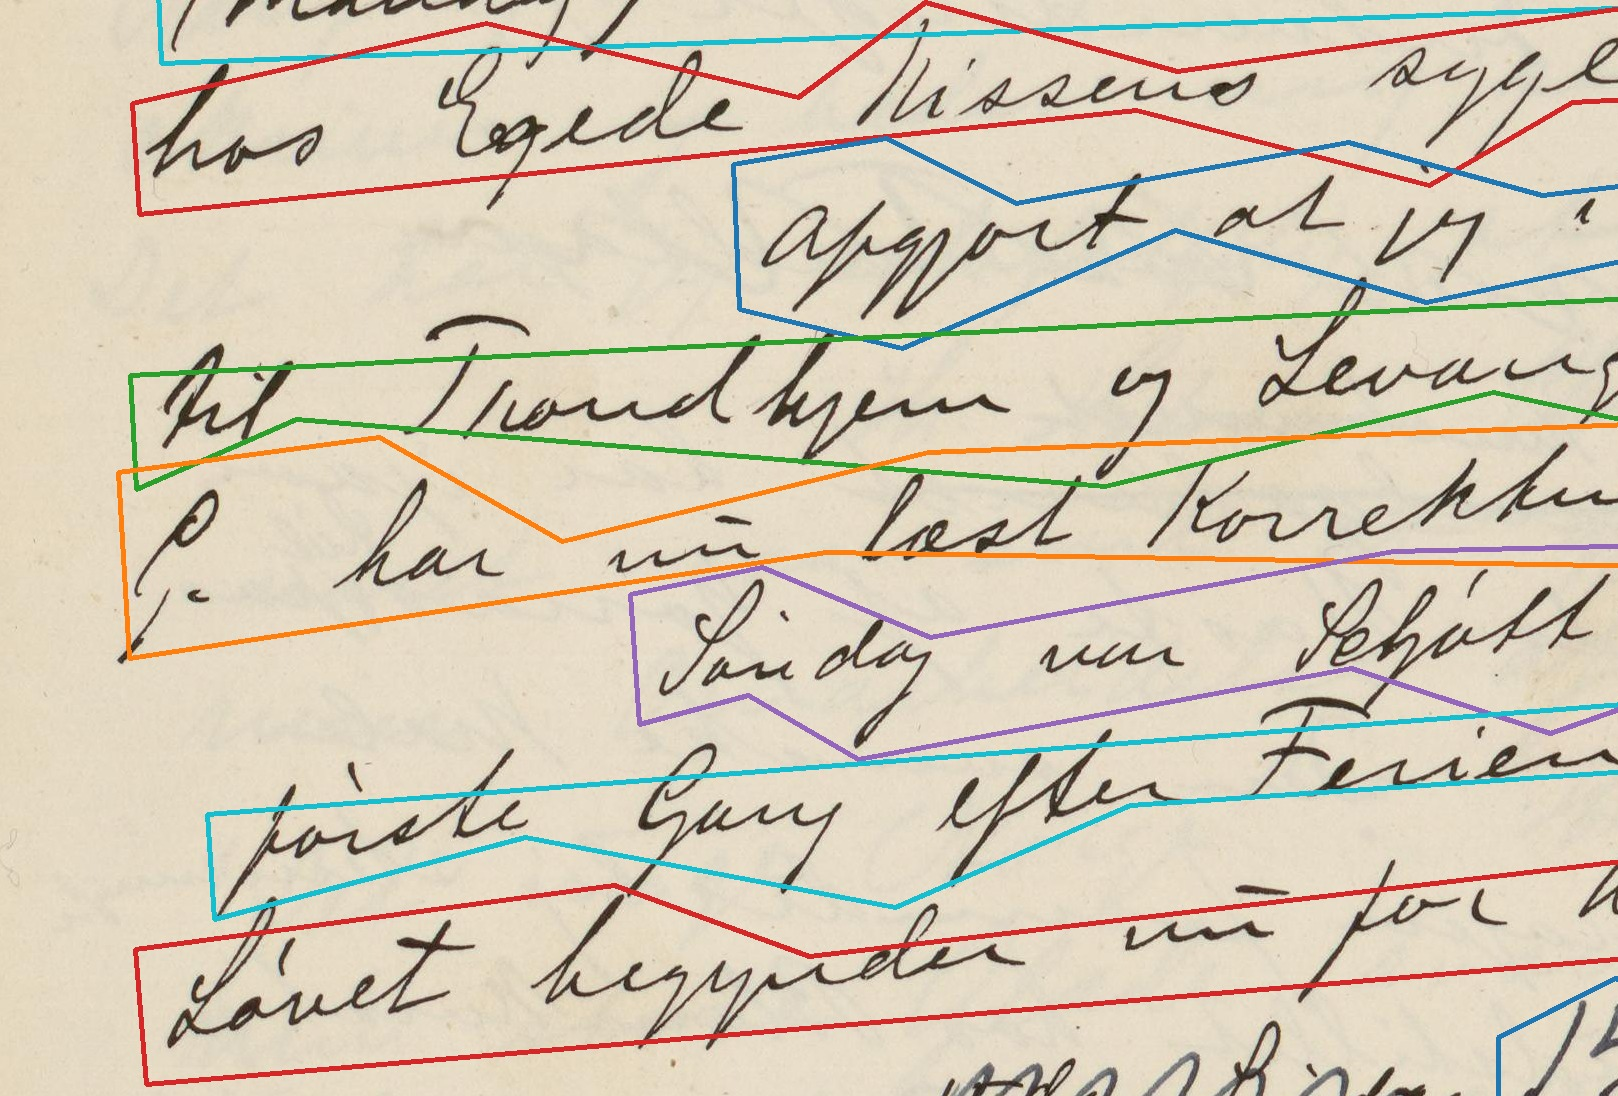
\includegraphics[width=\linewidth,height=4.2cm,keepaspectratio]{graphics/rq3gt_NorHand_v3.jpg}\caption{NorHand v3.}\end{subfigure}

    \medskip
    \begin{subfigure}[t]{\linewidth}\centering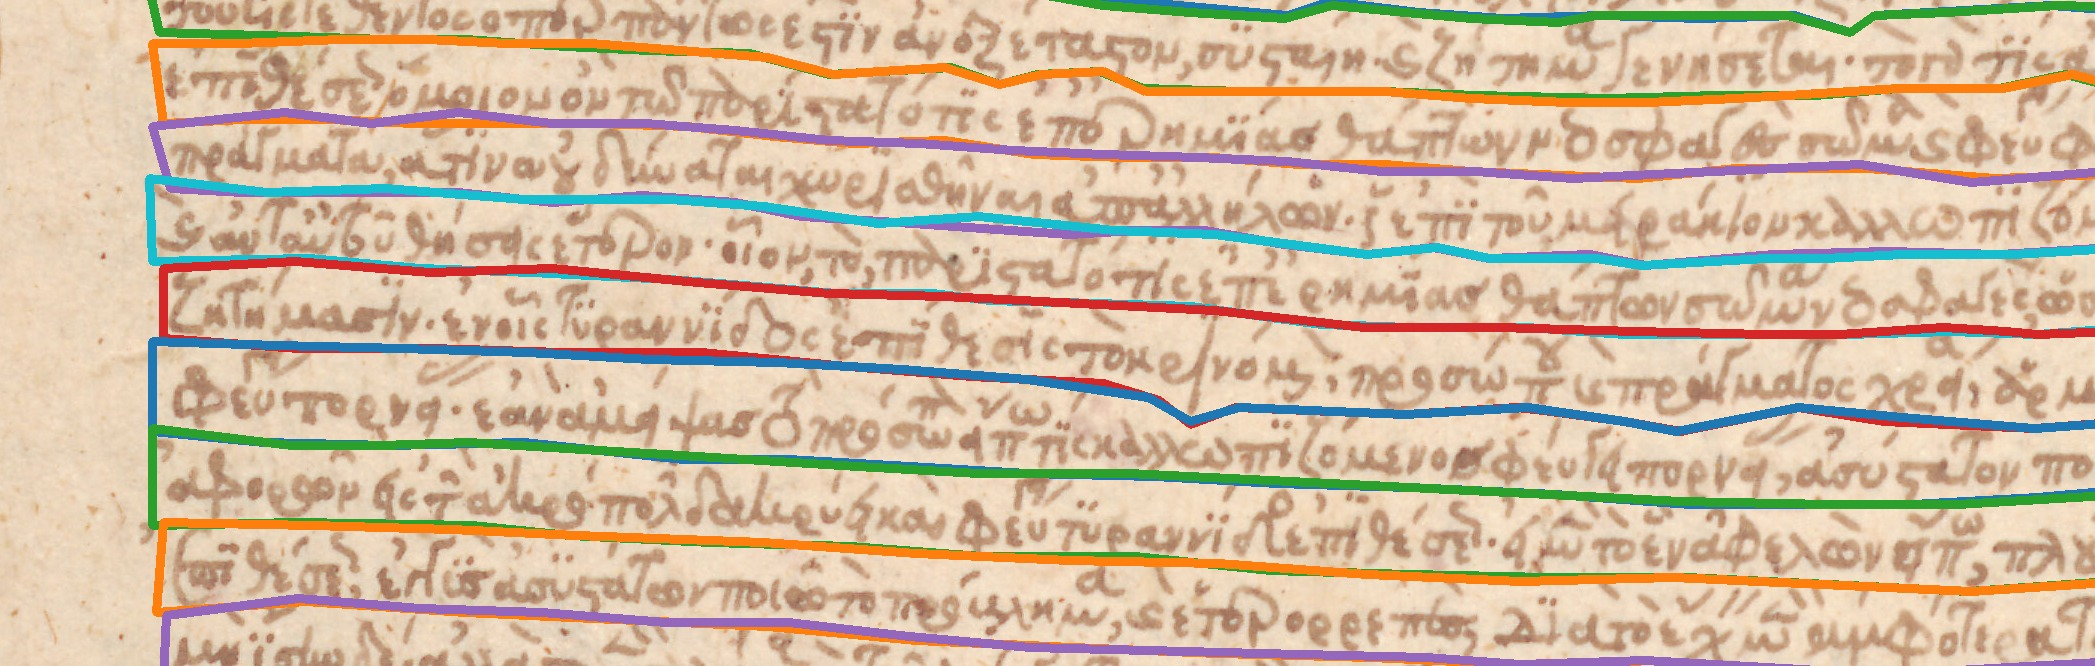
\includegraphics[width=\linewidth]{graphics/rq3gt_Phil_gr_130.jpg}\caption{Phil.\ gr.\ 130.}\end{subfigure}
    \caption[Training-page crops of the seven cross-collection datasets]{Training-page crops of the seven cross-collection datasets with ground-truth line polygons. Generated from Pinkas~\cite{Barakat2019Pinkas}, ONB Cod.\ Syr.\ 1~\cite{AboudIshac2025ONBSyr1}, RASAM~\cite{VidalGorene2021RASAM}, RASM2018/2019~\cite{KeinanSchoonbaert2019RASM}, GRPOLY-DB~\cite{Gatos2015GRPOLY}, NorHand v3~\cite{Beyer2023NorHand}, and Phil.\ gr.\ 130~\cite{SindlevAndersen2026PhilGrGT}.}
    \label{fig:rq3-collections}
\end{figure}

\glsunset{dr}\glsunset{ra}
\section{Evaluation Metrics}
\label{metrics}

Evaluation uses five metrics computed with the DIVA Line Segmentation Evaluator~\cite{diva_tool}: Pixel Intersection over Union (Pixel IU), Line Intersection over Union (Line IU), Detection Rate (DR), Recognition Accuracy (RA), and F-Measure (FM). For U-DIADS-TL, the FEST evaluator is used instead~\cite{Zottin_2025_FEST}.

\begin{enumerate}
    \item \Gls{pixeliu} measures the overlap between predicted and ground-truth foreground pixels:
    \[\text{Pixel IU} = \frac{TP}{TP + FP + FN}.\]

    \item \Gls{lineiu} applies the same intersection-over-union principle at the text-line level:
    \[\text{Line IU} = \frac{TP}{TP + FP + FN}.\]
    Here, $TP$, $FP$, and $FN$ denote correctly detected, extra, and missed lines, respectively. A prediction is correct when both its pixel precision and recall are at least $75\%$.

    \item \Gls{dr} measures the proportion of ground-truth lines that are matched:
    \[\text{DR} = \frac{M}{N_1},\]
    where $M$ is the number of matched lines and $N_1$ is the number of ground-truth lines.

    \item \Gls{ra} measures the proportion of predicted lines that are matched:
    \[\text{RA} = \frac{M}{N_2},\]
    where $N_2$ is the number of predicted lines.

    \item \Gls{fm} is the harmonic mean of DR and RA:
    \[\text{FM} = \frac{2\cdot\text{DR}\cdot\text{RA}}{\text{DR}+\text{RA}}.\]
\end{enumerate}

\section{Experiment Configurations}

The experiments answer the three \glspl{rq}. \Gls{rq}~1 compares the pipelines, encoders, and initializations on the complete benchmark partitions, \gls{rq}~2 reduces the number of training pages, and \gls{rq}~3 applies the models to collections that were not seen during training.

\subsection{Training Setup}
\label{sec:training-setup}\label{sec:training-semantic}\label{sec:training-two-stage}\label{sec:training-mask-rcnn}\label{sec:training-center-line}

All pipelines are trained on the same instance representation of the \gls{gt}: every line polygon of DIVA-HisDB, CATMuS, and the cross-collection datasets, and every connected component of a U-DIADS-TL mask, becomes an instance mask and a \gls{bbox}. U-DIADS-TL and DIVA-HisDB keep their benchmark partitions, and in \gls{rq}~2 the training pages are selected from the training pool of each DIVA-HisDB manuscript while the validation pages stay the same. For every pipeline, the checkpoint, the thresholds, and the postprocessing parameters are selected on the validation pages, and all runs use the same seed. The transfer experiments of \gls{rq}~3 use the settings of Section~\ref{sec:cross-generalization}.

Table~\ref{tab:training-settings} lists the training settings of the five networks. The detectors use only photometric augmentation, so that the instance geometry stays aligned with the page. Since RT-DETR is trained with a batch size of one, its BatchNorm layers are frozen. Mask R-CNN uses anchors adapted to long and thin text lines and identical heads for all encoders. Its box and mask predictors are reinitialized for the text line class, while the other heads keep their \gls{coco} initialization. The center-line model is trained on page crops rescaled to a common line thickness and is decoded as described in Section~\ref{sec:rq3-center-line}.

\begin{table}[htbp]
    \centering
    \caption{Training settings of the networks in \gls{rq}~1 and \gls{rq}~2.}
    \label{tab:training-settings}\label{tab:rq3-center-line-settings}
    \scriptsize
    \setlength{\tabcolsep}{3pt}
    \begin{tabular}{@{}llllll@{}}
        \toprule
        & U-Net & Center-line & RT-DETR & BBox U-Net & Mask R-CNN \\
        \midrule
        Encoder & 3 families & ConvNeXt-Tiny & 3 families & ResNet-34 & 3 families \\
        Input & \(448^2\) crops & \(512^2\) crops\(^{a}\) & page, \(1152^2\) & \(1024\times256\) crops & page, \(704^2\)/\(1024^2\)\(^{b}\) \\
        Length & \(\le\)100 epochs\(^{c}\) & 1,500/800 steps\(^{b}\) & 100 epochs & 50 epochs & 30/200 epochs\(^{b}\) \\
        Batch size & 4 & 4 & 1 (\(\times\)2 accum.) & 4 & 1 \\
        Learning rate\(^{d}\) & \(10^{-3}\) / \(10^{-4}\) & \(3\cdot10^{-4}\) / \(10^{-4}\) & \(10^{-4}\) & \(3\cdot10^{-4}\) & \(10^{-3}\) / \(10^{-4}\) \\
        Schedule & cosine & one-cycle & constant & constant & cosine \\
        Loss & BCE + Dice & BCE + Dice, \(L_1\) & RT-DETR loss & BCE / Tversky / SV & Mask R-CNN loss \\
        Augmentation & flip, rotation, B/C & B/C, blur & color jitter & B/C, affine, noise & color jitter \\
        Checkpoint & val.\ pixel \gls{iou} & final & val.\ box mAP & val.\ Dice & val.\ split \\
        \bottomrule
    \end{tabular}
    \par\smallskip
\end{table}

The BBox U-Net is trained separately from the detectors on \gls{gt} line crops, so that the same model can segment the boxes of both detectors. Three losses are compared for it: \gls{bce}, the Tversky loss~\cite{salehi2017tversky}, which weights missed foreground pixels more strongly than false positives, and the connectivity-preserving SuperVoxel loss~\cite{grim2025supervoxel}, which penalizes split and merged components. In \gls{rq}~1, the detector comparisons use a fixed BBox U-Net, trained with the Tversky loss on U-DIADS-TL and with BCE on DIVA-HisDB, and the loss study is reported in Appendix~\ref{app:rq1-extra}.

\label{sec:training-pretraining}
Two initializations of Section~\ref{sec:initializations} require an additional training stage before few-shot fine-tuning: the distillation on cBAD 2019 (Table~\ref{tab:distillation}) and the supervised pretraining on CATMuS (Table~\ref{tab:catmus-pretraining}). Because of limited computational resources, the distillation schedules are shorter than recommended by LightlyTrain~\cite{lightlytrain-distillation}.

\begin{table}[htbp]
    \centering
    \caption{Distillation on cBAD 2019.}
    \label{tab:distillation}
    \footnotesize
    \setlength{\tabcolsep}{4pt}
    \begin{tabular}{@{}ll@{}}
        \toprule
        Setting & Value \\
        \midrule
        Data & 3,021 unlabeled cBAD 2019 pages \\
        Teacher & DINOv3 ViT-B/16 \\
        Students & ConvNeXt-Tiny, PVTv2-B2, ViT-Small (random initialization) \\
        Length & 1,100 epochs (ConvNeXt-Tiny), 300 epochs (PVTv2-B2, ViT-Small) \\
        Input / batch size & \(224^2\) random crops / 128 (gradient accumulation) \\
        Optimizer & AdamW, peak learning rate \(1.44\cdot10^{-4}\), weight decay 0.04\(^{a}\) \\
        Schedule & cosine with 10 warm-up epochs \\
        Augmentation & random resized crops, flip, color jitter, grayscale, blur \\
        Checkpoint & last epoch \\
        \bottomrule
    \end{tabular}
    \par\smallskip
    \parbox{0.86\linewidth}{\scriptsize \(^{a}\)Excluding bias, normalization, and token parameters.}
\end{table}

\begin{table}[htbp]
    \centering
    \caption{Pretraining on CATMuS Medieval.}
    \label{tab:catmus-pretraining}
    \footnotesize
    \setlength{\tabcolsep}{4pt}
    \begin{tabular}{@{}llll@{}}
        \toprule
        & Mask R-CNN & RT-DETR & Center-line \\
        \midrule
        Data & 1,335 / 191 pages\(^{a}\) & 1,335 / 191 pages\(^{a}\) & 1,334 pages\(^{a}\) \\
        Supervision & line masks & line boxes & center lines, ends, distances \\
        Length & 30 epochs & 10 epochs & 12,000 steps \\
        Input & \(704^2\) & \(1152^2\) & \(512^2\) crops\(^{b}\) \\
        Batch size & 1 & 1 (\(\times\)2 accum.) & 4 \\
        Learning rate\(^{c}\) & \(10^{-3}\) / \(10^{-4}\) & \(10^{-4}\) & \(3\cdot10^{-4}\) / \(10^{-4}\) \\
        Schedule & cosine & constant & one-cycle \\
        Augmentation & color jitter & color jitter & B/C, blur \\
        Checkpoint & val.\ mask AP@0.5 & val.\ box AP@[0.5:0.95] & final \\
        \bottomrule
    \end{tabular}
    \par\smallskip
\end{table}

\subsection{Page Selection Setup}
\label{sec:page-selection-setup}

The page selection of \gls{rq}~2 is applied to DIVA-HisDB, since only its manuscripts provide a pool of twenty training pages, whereas U-DIADS-TL provides three. The strategies of Section~\ref{sec:shot-sampling} choose \(k\in\{1,3,5,10,15\}\) pages from the twenty training pages of each DIVA-HisDB manuscript. For the embedding-based strategies, each page is resized to \(720\times720\) pixels and ImageNet-normalized, and each feature dimension is standardized across the candidate pool.

\begin{figure}[htbp]
    \centering
    \begin{subfigure}[t]{0.49\linewidth}\centering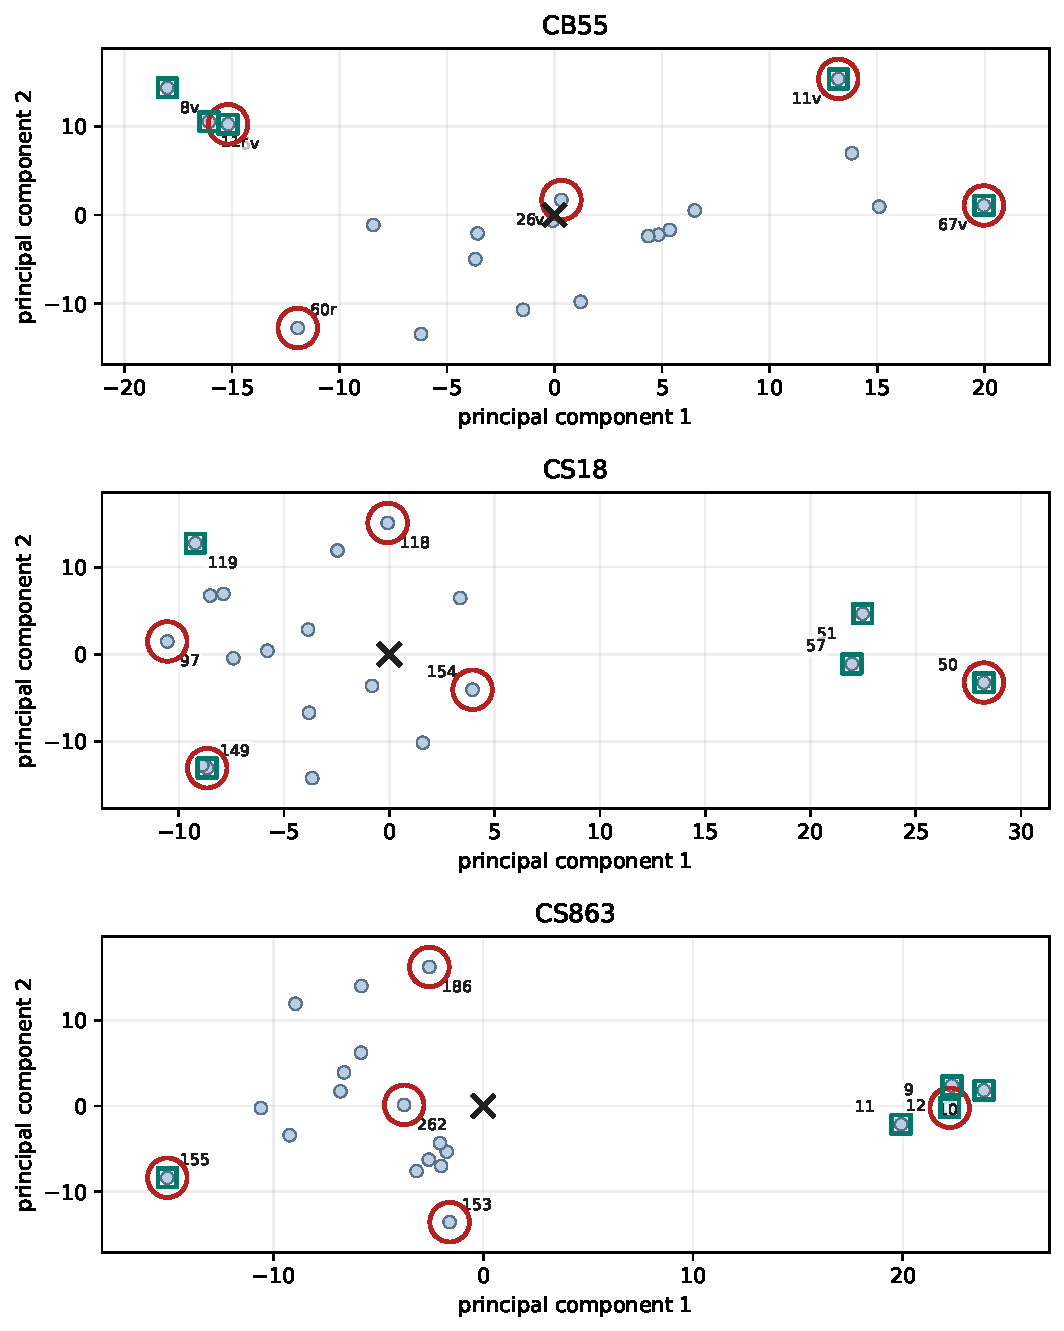
\includegraphics[width=\linewidth]{graphics/shot_sampling_pca.pdf}\caption{\Gls{pca} projections.}\label{fig:shot-sampling-pca}\end{subfigure}\hfill
    \begin{subfigure}[t]{0.49\linewidth}\centering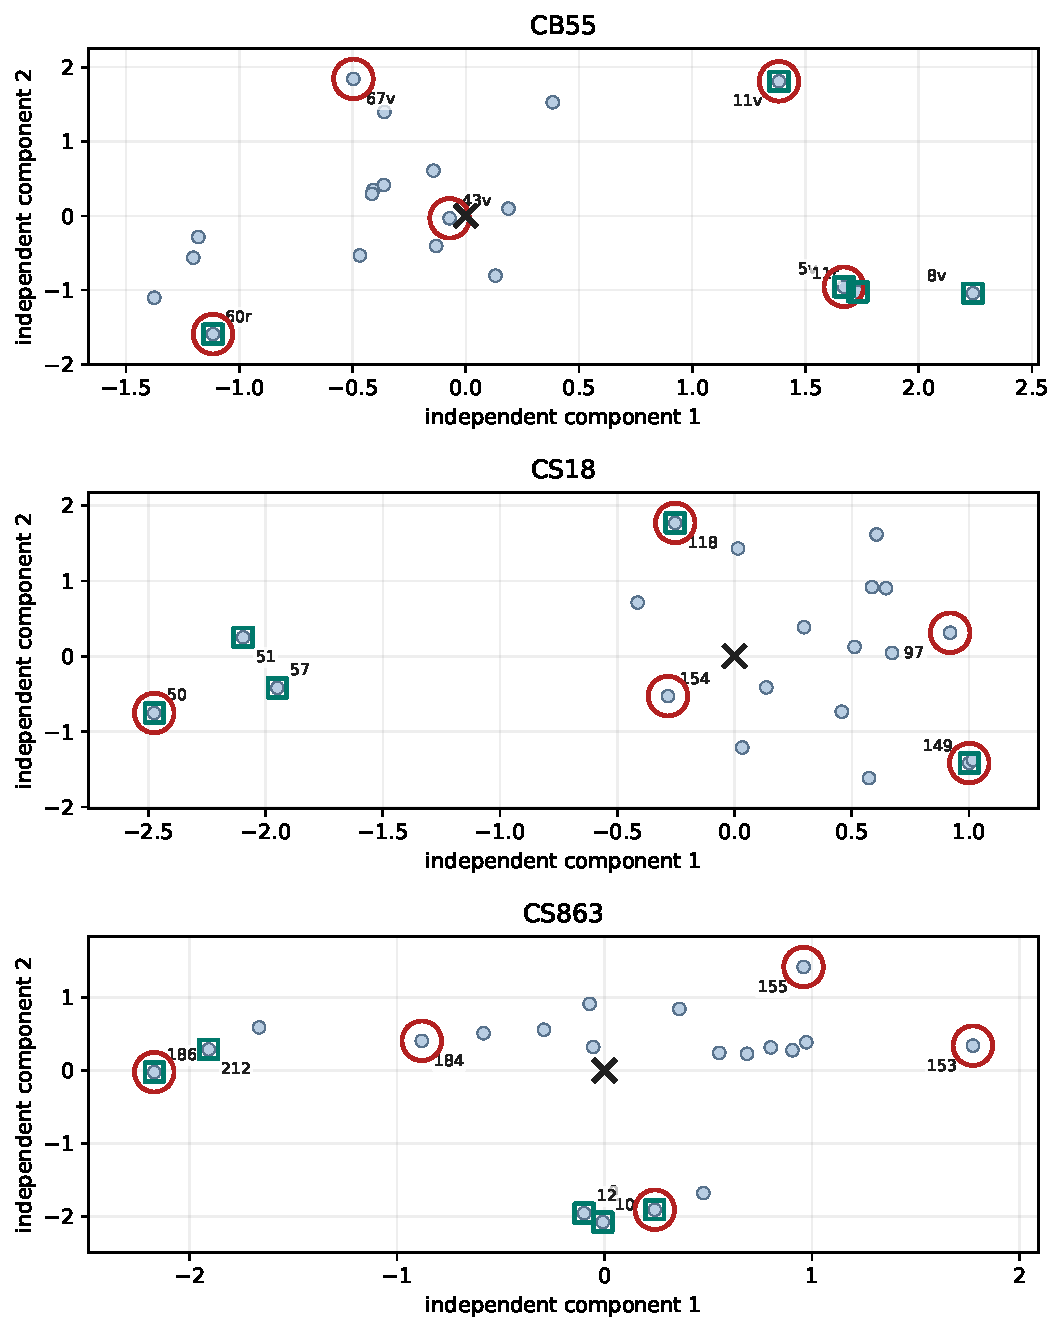
\includegraphics[width=\linewidth]{graphics/shot_sampling_ica.pdf}\caption{\Gls{ica} projections.}\label{fig:shot-sampling-ica}\end{subfigure}
    \caption[Page projections for five-shot page selection]{Two-dimensional projections of the twenty training pages per DIVA-HisDB manuscript (rows: CB55, CS18, CS863) with five-shot selections: max--min (red circles), farthest from centroid (green squares), centroid (black crosses). Generated from DIVA-HisDB~\cite{diva_hisdb}.}
    \label{fig:shot-sampling}
\end{figure}

\subsection{Cross-Collection Transfer}
\label{sec:cross-generalization}

\Gls{rq}~3 examines whether a model trained on a few pages of one or more collections transfers to a collection that it has never seen during training. For this purpose, it uses the seven cross-collection datasets of Section~\ref{sec:datasets}.

\label{sec:data-partitions}

Five of the seven cross-collection datasets, ONB Cod.\ Syr.\ 1, RASAM, RASM2018/2019, Phil.\ gr.\ 130, and GRPOLY-DB, are released without an official partition. To give all seven cross-collection datasets the same conditions, each of them is partitioned once with three pages are drawn for training, 10\% of the pages for validation, and the remaining pages form the test set. Pinkas and NorHand v3 keep their official test sets and hold their training and validation pages from the official training part, which for NorHand v3 is a random subset of 30 pages. 

All experiments use the center-line model (Section~\ref{sec:rq3-center-line}) and Mask R-CNN (Section~\ref{sec:mask-rcnn-method}). Table~\ref{tab:rq3-training-settings} lists the model, augmentation, and optimization settings. The configuration is selected by the mean source-validation \gls{fm} among cumulative modifications of a baseline on nine source--target pairs, so that no target test page influences the choice. Score and mask thresholds are selected by validation \gls{fm}, and \gls{pixeliu} decides between settings with the same \gls{fm}.

\begin{table}[htbp]
    \centering
    \caption{Settings of the transfer experiments.}
    \label{tab:rq3-training-settings}
    \footnotesize
    \setlength{\tabcolsep}{4pt}
    \begin{tabular}{@{}lll@{}}
        \toprule
        & Mask R-CNN & Center-line \\
        \midrule
        Initialization & ConvNeXt-Tiny, CATMuS & ConvNeXt-Tiny, CATMuS or cBAD \\
        Input & \(1152^2\) canvas & \(512^2\) crops (Table~\ref{tab:training-settings}) \\
        Length & 50 epochs & 3,000 steps \\
        Batch size & 1 & 4 \\
        Learning rate\(^{a}\) & \(10^{-3}\) / \(10^{-4}\) & \(3\cdot10^{-4}\) / \(10^{-4}\) \\
        Schedule & cosine & one-cycle \\
        Augmentation & scale jitter\(^{b}\), photometric & B/C, blur \\
        Anchors & 32--512 pixels; ratios 0.05--1.0 & -- \\
        Thresholds & score \(\{0.3,0.5,0.7,0.9\}\), mask \(\{0.3,0.5\}\)\(^{c}\) & -- \\
        \bottomrule
    \end{tabular}
    \par\smallskip
    \end{table}

At inference, masks are assigned in descending confidence order and restored to page resolution. The largest contour of each mask defines its text line polygon, and points near its lowest point define the baseline, using the tolerance in Table~\ref{tab:rq3-training-settings}. Predictions are not clipped to a main-text region, because the collections do not provide one.

\label{sec:wiseft}

Fine-tuning on a few annotated pages adapts a pretrained model to these pages but can reduce the robustness that it gained during pretraining. Therefore, it is checked whether \gls{wiseft}~\cite{wortsman2022wiseft} improves the transfer. It requires no additional training: the weights of the pretrained and the fine-tuned model are linearly interpolated,
\begin{equation}
    \theta = (1-\alpha)\,\theta_{\mathrm{pre}} + \alpha\,\theta_{\mathrm{ft}},
    \label{eq:wiseft}
\end{equation}
where \(\theta_{\mathrm{pre}}\) and \(\theta_{\mathrm{ft}}\) denote the pretrained and fine-tuned weights, and \(\alpha\) is the interpolation weight. A weight of \(\alpha=0\) gives the pretrained model and \(\alpha=1\) the fine-tuned model. The CATMuS-pretrained center-line model uses \(\alpha=0.5\), which was fixed before the evaluation, whereas Mask R-CNN and the cBAD-encoder center-line model use the fine-tuned weights. To measure the effect of \(\alpha\), both CATMuS-pretrained models are additionally evaluated in single-collection transfer with \(\alpha\in\{0,0.25,0.5,0.75,1\}\).

Transfer is measured in three settings:
\begin{itemize}
    \item \textbf{Zero-shot.} The CATMuS-pretrained model is applied without fine-tuning, using the fixed thresholds in Table~\ref{tab:rq3-training-settings}.
    \item \textbf{Single-collection transfer.} One model is trained on the three training pages of each collection, its thresholds are selected on the validation pages of that collection, and it is applied unchanged to all seven test sets. The diagonal of the resulting \(7\times7\) matrix is the in-domain result, and the off-diagonal cells measure zero-shot transfer.
    \item \textbf{\Gls{loco} transfer.} For each held-out collection, a \gls{loco} model is trained on \(k\in\{1,2,3\}\) pages from each of the six other collections, that is, on 6, 12, or 18 pages (\gls{loco}-1, \gls{loco}-2, and \gls{loco}-3). The page sets are nested and taken from the single-collection training pages. The thresholds are selected on up to three validation pages per source collection, so the held-out collection takes no part in training or selection. The result is compared with the in-domain result and with the best off-diagonal single-collection entry of the same column, which overestimates a source chosen in advance because it is identified on test results.
\end{itemize}

% Dataset figures removed for now; restore by uncommenting.
% \begin{figure}[H]
%     \centering
%     \includegraphics[width=0.9\linewidth]{graphics/udiads_examples_fest.png}
%     \caption{U-DIADS-TL pages with their line instances (Latin2, Latin14396, Syriaque 341), reproduced from~\cite{Zottin_2025_FEST}.}
%     \label{fig:udiads-examples}
% \end{figure}

% \begin{figure}[H]
%     \centering
%     \begin{subfigure}[t]{0.31\linewidth}
%         \centering
%         \includegraphics[width=\linewidth,height=0.31\textheight,keepaspectratio]{graphics/diva_cb55_page.png}
%         \caption{CB55 page.}
%     \end{subfigure}\hfill
%     \begin{subfigure}[t]{0.31\linewidth}
%         \centering
%         \includegraphics[width=\linewidth,height=0.31\textheight,keepaspectratio]{graphics/diva_csg18_page.png}
%         \caption{CSG18 page.}
%     \end{subfigure}\hfill
%     \begin{subfigure}[t]{0.31\linewidth}
%         \centering
%         \includegraphics[width=\linewidth,height=0.31\textheight,keepaspectratio]{graphics/diva_csg863_page.png}
%         \caption{CSG863 page.}
%     \end{subfigure}
%
%     \medskip
%
%     \begin{subfigure}[t]{0.31\linewidth}
%         \centering
%         \includegraphics[width=\linewidth,height=0.20\textheight,keepaspectratio]{graphics/diva_cb55_detail.png}
%         \caption{CB55 detail.}
%     \end{subfigure}\hfill
%     \begin{subfigure}[t]{0.31\linewidth}
%         \centering
%         \includegraphics[width=\linewidth,height=0.20\textheight,keepaspectratio]{graphics/diva_csg18_detail.png}
%         \caption{CSG18 detail.}
%     \end{subfigure}\hfill
%     \begin{subfigure}[t]{0.31\linewidth}
%         \centering
%         \includegraphics[width=\linewidth,height=0.20\textheight,keepaspectratio]{graphics/diva_csg863_detail.png}
%         \caption{CSG863 detail.}
%     \end{subfigure}
%     \caption{DIVA-HisDB pages and details, reproduced from De Nardin et al.~\cite{De_Nardin_2023} (DIVA-HisDB~\cite{diva_hisdb}).}
%     \label{fig:diva-examples}
% \end{figure}

% \begin{figure}[H]
%     \centering
%     \begin{subfigure}[t]{0.32\linewidth}
%         \centering
%         \includegraphics[width=\linewidth]{graphics/rq3_pinkas.jpg}
%         \caption{Pinkas.}
%     \end{subfigure}\hfill
%     \begin{subfigure}[t]{0.32\linewidth}
%         \centering
%         \includegraphics[width=\linewidth]{graphics/rq3_onb_cod_syr_1.jpg}
%         \caption{ONB Cod.\ Syr.\ 1.}
%     \end{subfigure}\hfill
%     \begin{subfigure}[t]{0.32\linewidth}
%         \centering
%         \includegraphics[width=\linewidth]{graphics/rq3_rasam.jpg}
%         \caption{RASAM.}
%     \end{subfigure}
%
%     \medskip
%
%     \begin{subfigure}[t]{0.32\linewidth}
%         \centering
%         \includegraphics[width=\linewidth]{graphics/rq3_phil_gr_130.jpg}
%         \caption{Phil.\ gr.\ 130.}
%     \end{subfigure}\hfill
%     \begin{subfigure}[t]{0.32\linewidth}
%         \centering
%         \includegraphics[width=\linewidth]{graphics/rq3_norhand_v3.jpg}
%         \caption{NorHand v3.}
%     \end{subfigure}\hfill
%     \begin{subfigure}[t]{0.32\linewidth}
%         \centering
%         \includegraphics[width=\linewidth]{graphics/rq3_grpoly-db_handwritten.jpg}
%         \caption{GRPOLY-DB Handwritten.}
%     \end{subfigure}
%
%     \medskip
%
%     \begin{subfigure}[t]{0.32\linewidth}
%         \centering
%         \includegraphics[width=\linewidth]{graphics/rq3_rasm2018_2019.jpg}
%         \caption{RASM2018/2019.}
%     \end{subfigure}
%     \caption[Example pages of the seven RQ3 collections]{Example pages of the seven RQ3 collections with ground-truth line polygons. Generated from Pinkas~\cite{Barakat2019Pinkas}, ONB Cod.\ Syr.\ 1~\cite{AboudIshac2025ONBSyr1}, RASAM~\cite{VidalGorene2021RASAM}, Phil.\ gr.\ 130~\cite{SindlevAndersen2026PhilGrGT}, NorHand v3~\cite{Beyer2023NorHand}, GRPOLY-DB~\cite{Gatos2015GRPOLY}, and RASM2018/2019~\cite{KeinanSchoonbaert2019RASM}.}
%     \label{fig:dataset-examples}
% \end{figure}
